%--------preamble----------

\documentclass[letterpaper,11pt]{article}
\usepackage{graphicx}
\graphicspath{ {images/} }             %image path
\usepackage{wrapfig}
\newlength{\outerbordwidth}
\pagestyle{empty}
\raggedbottom
\raggedright
\usepackage[svgnames]{xcolor}
\usepackage{framed}
\usepackage{tocloft}
\usepackage{amsmath}
\usepackage{etoolbox}
\robustify\cftdotfill

%-----------------------------------------------------------
%Edit these values as you see fit
\setlength{\outerbordwidth}{3pt}  % Width of border outside of title bars
\definecolor{shadecolor}{gray}{0.75}  % Outer background color of title bars (0 = black, 1 = white)
\definecolor{shadecolorB}{gray}{0.93}  % Inner background color of title bars

%-------------------page setup----------------------------
%Margin setup
\setlength{\evensidemargin}{-0.25in}
\setlength{\headheight}{-0.25in}
\setlength{\headsep}{0in}
\setlength{\oddsidemargin}{-0.25in}
\setlength{\paperheight}{11in}
\setlength{\paperwidth}{8.5in}
\setlength{\tabcolsep}{0in}
\setlength{\textheight}{9.75in}
\setlength{\textwidth}{7in}
\setlength{\topmargin}{-0.3in}
\setlength{\topskip}{0in}
\setlength{\voffset}{0.1in}

%-------------------------------------------------

%-----------define macro-----------

\newcommand{\Sep}{\vspace{1.5em}}
\newcommand{\SmallSep}{\vspace{0.5em}}

\newenvironment{AboutMe}
{\ignorespaces\textbf{\color{RoyalBlue} About me}}
{\Sep\ignorespacesafterend}

\newcommand{\CVSection}[1]
{\Large\textbf{#1}\par
	\SmallSep\normalsize\normalfont}

\newcommand{\CVItem}[1]
{\textbf{\color{RoyalBlue} #1}}

%---------------------------------

\newcommand{\resitem}[1]{\item #1 \vspace{-2pt}}
\newcommand{\resheading}[1]{\vspace{8pt}
	\parbox{\textwidth}{\setlength{\FrameSep}{\outerbordwidth}
		\begin{shaded}
			
			\setlength{\fboxsep}{0pt}\framebox[\textwidth][l]{\setlength{\fboxsep}{4pt}\fcolorbox{shadecolorB}{shadecolorB}{\textbf{\sffamily{\mbox{~}\makebox[6.762in][l]{\large #1} \vphantom{p\^{E}}}}}}
		\end{shaded}
	}\vspace{-5pt}
}

\newcommand{\ressubheading}[4]{
	\begin{tabular*}{6.5in}{l@{\cftdotfill{\cftsecdotsep}\extracolsep{\fill}}r}
		\textbf{#1} & #2 \\
		\textit{#3} & \textit{#4} \\
	\end{tabular*}\vspace{-6pt}}
%---------------------------------------------------

%----------body starts------------
\begin{document}

%---------------------Personal Information---------
%---------------------Image-----------------
\begin{wrapfigure}{r}{4.5cm}
	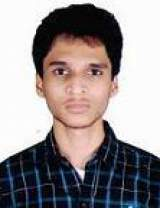
\includegraphics[width=2.5cm]{PHOTO}
\end{wrapfigure} 

%------------------------------------------
\textbf{}  \\
\textbf{{\Large Abhishek Rai}}  \\
Email \hspace{0.2cm}  : a.rai@somaiya.edu \\
Contact : 9969961337 \\
Address : B-305, building no.44 \\
\hspace{1.8cm}Tilak Nagar, Mumbai - 400089 \\ 
Linkedin : www.linkedin.com/in/abhishek-rai-814870145


%\textbf{}  \\
%-----------------------------------	

%------------------Objective---------------
\textbf{}  \\
\CVSection{Objective}
To work on projects that involve using concepts of design, machining and testing in order to enhance a process of a system. In search of position at an innovative firm.  \\

%-------------Education---------------------------
\textbf{}  \\
\CVSection{Education}

\begin{table}[h!]
	\begin{center}
		\begin{tabular}{l|c|r|l} % <-- Alignments: 1st column left, 2nd middle and 3rd right, with vertical lines in between
			\hspace{0.2cm}\textbf{Year}\hspace{0.2cm} &\hspace{0.2cm} \textbf{Degree/Certificate}\hspace{0.2cm} &\hspace{0.2cm} \textbf{Institute}\hspace{2.3cm} &\hspace{0.2cm} \textbf{CGPA / Percentage}\hspace{0.2cm}\\
			\hline
			2012 & \hspace{0.2cm} Secondary School Certificate \hspace{0.2cm} & \hspace{0.2cm}Swami Vivekanand High School\hspace{1.7cm} & \hspace{1.2cm} 86.73\% \hspace{0.2cm}\\
			2014 & \hspace{0.2cm} Higher Secondary School Certificate \hspace{0.2cm} & \hspace{0.2cm}R.J Junior College\hspace{1.7cm} & \hspace{1.2cm} 84.46\% \hspace{0.2cm}\\
			2014 & \hspace{0.2cm} 1st Semester Btech Mech \hspace{0.2cm} & \hspace{0.2cm}K.J. Somaiya College of Engineering\hspace{0.2cm} & \hspace{1.2cm} 8.69 \hspace{0.2cm}\\
			2015 & \hspace{0.2cm} 2nd Semester Btech Mech \hspace{0.2cm} & \hspace{0.2cm}K.J. Somaiya College of Engineering\hspace{0.2cm} & \hspace{1.2cm} 8.19 \hspace{0.2cm}\\
			2015 & \hspace{0.2cm} 3rd Semester Btech Mech \hspace{0.2cm} & \hspace{0.2cm}K.J. Somaiya College of Engineering\hspace{0.2cm} & \hspace{1.2cm} 7.57 \hspace{0.2cm}\\
			2016 & \hspace{0.2cm} 4th Semester Btech Mech \hspace{0.2cm} & \hspace{0.2cm}K.J. Somaiya College of Engineering\hspace{0.2cm} & \hspace{1.2cm} 7.98 \hspace{0.2cm}\\
			2016 & \hspace{0.2cm} 5th Semester Btech Mech \hspace{0.2cm} & \hspace{0.2cm}K.J. Somaiya College of Engineering\hspace{0.2cm} & \hspace{1.2cm} 7.82 \hspace{0.2cm}\\
			2017 & \hspace{0.2cm} 6th Semester Btech Mech \hspace{0.2cm} & \hspace{0.2cm}K.J. Somaiya College of Engineering\hspace{0.2cm} & \hspace{1.2cm} 7.28 \hspace{0.2cm}\\
			2017 & \hspace{0.2cm} 7th Semester Btech Mech \hspace{0.2cm} & \hspace{0.2cm}K.J. Somaiya College of Engineering\hspace{0.2cm} & \hspace{1.2cm} 8.08 \hspace{0.2cm}\\
			
		\end{tabular}
	\end{center}
\end{table}
\textbf{}  \\
\textbf{}  \\

%--------------------------Projects------------------------------
\CVSection{Projects}

\textbf{Autonomous Water Rover} (July 2017 - Present): \\
An autonomous water surface vehicle aimed for still water body monitoring and surveillance, along with applications like depth mapping, fish finding.  \\

\textbf{}  \\
\textbf{Robo-Rehab} (December 2017 - Present): \\
An automated continuous passive motion device for the arm to aid physiotherapists in rehabilitation of paralysis/stroke victims and compile statistical report to track the growth of muscle strength.
\textbf{}  \\
\textbf{}  \\

\textbf{Pole climbing robot} (December 2017 - March 2018): \\
Pneumatic based pole climbing robot capable of translating linearly.
\textbf{}  \\
\textbf{}  \\


\textbf{4-axis robotic arm} (2016): \\
A 4-axis articulated robot controlled using forward kinematics.
\textbf{}  \\
\textbf{}  \\


\textbf{Robocon} (November 2015 - March 2016)\\
Designed and fabricated eco and hybrid robot to perform the tasks specified by ROBOCON theme.
\textbf{}  \\
\textbf{}  \\


\textbf{Robocon} (November 2016 - March 2017)\\
Designed and fabricated a frisbee launching robot.
\textbf{}  \\
\textbf{}  \\
\textbf{}  \\

%-----------------------Internship and Trainings---------
\CVSection{Experience: KJSCE ROBOCON (OFFICIAL ROBOTIC TEAM OF KJSCE)}
\textbf{Technical Head} (May 2016 - April 2017) \\


\begin{itemize}
	\item Developed prototype components, assemblies and tooling
	\item Managed design and manufacturing team to build proprietary process equipment within cost and time constraints
	\item  Created CAD models and drawing with motion and flow simulations
	\item Worked with various actuators including motors, pneumatics, linear actuators 
	\item Successfully designed and fabricated hybrid robot, wind powered eco robot and automated frisbee throwing robot
\end{itemize}
\textbf{}  \\

%-------------------Technical Skills----------------
\CVSection{Technical Skills}

\begin{enumerate}
	\item Software Platforms Used:\\
	\begin{itemize}
		\item Computer Aided Design (CAD):
		Soildworks(2017), Autodesk Inventor(2014)	
		\item FEA and simulation tools:
		Ansys(2016), Solidworks(2017),MATLAB(2016a)
		\item Programming languages: 
		C, C++, Python
		\item Others: 
		HTML, MySQL, Visual Studio
		
	\end{itemize}
	
	\item Hardware Machines : 
	\begin{itemize}
		\item Manufacturing: Lathe, CNC Lathe, Shaping machine
		\item Prototyping: 3D printer, Laser cutter
		
	\end{itemize}
\end{enumerate}
\textbf{}  \\

%---------------Soft Skills--------------------
\CVSection{Soft Skills}

\begin{itemize}
	\item Self Motivated
	\item Handles deatils  
	\item Keeps control over budget
	\item Defines needs
	\item Provides well-thought out solution
\end{itemize}
\textbf{}  \\

%----------------Extra Curricular Activities----------------
\CVSection{Extra-Curricular Activities}

\begin{itemize}
	\item Table Tennis
	\item Sketching 
	\item Volunteering in Education domain
	\item Trekking 
\end{itemize}
\textbf{}  \\
\textbf{}  \\

\end{document}